\documentclass{article}
% Numeric [1] citations with compressed ranges (e.g. [1--3]); standard for NeurIPS + natbib.
\PassOptionsToPackage{numbers,sort&compress}{natbib}
\usepackage[final]{neurips_2019}
\usepackage[T1]{fontenc}
\usepackage{graphicx}
\usepackage{xcolor}
\usepackage{float}
\usepackage{booktabs}
\usepackage{amsmath}
\usepackage{hyperref}

% Allow more flexible float placement to avoid large gaps
\renewcommand{\topfraction}{.85}
\renewcommand{\bottomfraction}{.7}
\renewcommand{\textfraction}{.15}
\renewcommand{\floatpagefraction}{.66}
\renewcommand{\dbltopfraction}{.66}
\renewcommand{\dblfloatpagefraction}{.66}
\setcounter{topnumber}{9}
\setcounter{bottomnumber}{9}
\setcounter{totalnumber}{20}
\setcounter{dbltopnumber}{9}

\setlength{\intextsep}{12pt plus 2pt minus 2pt}
\setlength{\textfloatsep}{12pt plus 2pt minus 4pt}

\newcommand{\note}[1]{\textcolor{blue}{#1}}

\title{
  Analysis of Retinal Representations\\in Vision Transformers\\
  \vspace{1em}
  \small{\normalfont Stanford CS375N Final Project}
}

\author{
  Xingyu (Brian) Zhou \\
  \texttt{xzhou25@stanford.edu}
}

\begin{document}

\maketitle

\begin{abstract}
The primate visual system processes information hierarchically, beginning at
the retina and passing through subcortical structures before reaching the
primary visual cortex (V1). While deep learning models have shown remarkable
success in matching cortical representations, their alignment with early,
pre-cortical visual processing stages remains less understood. This study
investigates the representational alignment between a biologically-constrained
Primate Retina Convolutional Neural Network (prCNN) and the self-supervised
Vision Transformer, DINOv2. Two central research questions are explored:
1)~How much subcortical processing occurs between the retina and V1? and
2)~Where does DINOv2 encode retinal-like features? By evaluating these models
against \texttt{TVSDV1} fMRI recordings using cross-validated ridge regression
and variance partitioning, this study finds that DINOv2 encoder~2 achieves the
best V1 match (ceiled $R^2 \approx 0.72$) and vastly outperforms the prCNN
(\texttt{conv1} ceiled $R^2 \approx 0.24$), indicating a substantial
computational role for subcortical processing; variance partitioning confirms
that DINOv2 accounts for unique V1 variance in over 91\% of voxels.
Using Linear Centered Kernel Alignment (CKA), cross-validated ridge regression,
and Representational Similarity Analysis (RSA, Spearman $r$) for direct
cross-model comparison on \texttt{TVSDStimulusTrainSet}, this study reveals
that DINOv2 encodes retinal-like features most strongly in its initial
embeddings layer and the first transformer block (encoder~0), with similarity
dropping sharply in deeper blocks. These findings highlight the emergence of
biologically plausible early visual representations in self-supervised
transformers, while also underscoring the substantial subcortical transformation
that separates retinal from cortical processing.
\end{abstract}

\section{Introduction}
A central goal in computational neuroscience is to build models that not only
functionally parallel biological neural structures but also accurately
predict biological neural responses. The biological visual
pathway begins at the retina, where photoreceptors capture light, bipolar
cells process it, and retinal ganglion cells (RGCs) transmit the signals via
the optic nerve to the lateral geniculate nucleus (LGN) and subsequently to
the primary visual cortex (V1).

Historically, Convolutional Neural Networks (CNNs) have been the standard for
modeling the visual cortex, with early layers mapping to V1 and deeper layers
mapping to inferior temporal (IT) cortex. Recently, Vision Transformers
(ViTs) trained with self-supervised learning, such as DINOv2, have
demonstrated highly robust and biologically plausible representations \cite{oquab_dinov2_2024}. 
However, fewer studies have explicitly analysed how these
large-scale foundation models encode subcortical neural structures like the retina.

This study investigates the representational similarities between DINOv2 
and a biologically-inspired primate retina CNN (prCNN) that is explicitly trained to predict the
firing rates of macaque RGCs \cite{alex_retina_cnn}. 
With BBScore \cite{noauthor_neuroailabbbscore_public_2026}, 
this study seeks to address two key questions through this comparison:
\begin{enumerate}
    \item \textbf{How much subcortical processing is there between the retina
    and V1?} By comparing how well the prCNN and DINOv2 layers predict V1 fMRI
    activity, this study can infer the extent of visual information processing that occurs
    after the retina and before V1.
    \item \textbf{Where does DINOv2 encode for the retina?} By directly
    comparing the internal representations of the prCNN and DINOv2, this study
    aims to locate where retinal-like features emerge within the transformer
    architecture.
\end{enumerate}

\section{Related Works}
Prior research has extensively compared deep neural networks to the primate
cortical visual system. Self-supervised Vision Transformers like DINOv2
\cite{oquab_dinov2_2024} have been shown to learn powerful visual features 
that achieve state-of-the-art alignment with V1 and higher visual areas. 
For the retina, CNN models have recently superseded traditional 
Linear-Nonlinear (LN) cascade models for accurately capturing the firing rates   
of numerically dominant RGC types in the macaque and human retina 
given visual stimuli \cite{alex_retina_cnn}.

This study contributes to the BBScore framework \cite{noauthor_neuroailabbbscore_public_2026}
in the following ways
\footnote{The codebase is available at \url{https://github.com/briansebzhou/bbscore_public}.}:
\begin{itemize}
    \item \textbf{Model Integration}: 
    This study introduced the biologically-constrained prCNN into the BBScore registry, 
    enabling standardized feature extraction and evaluation.
    \item \textbf{Benchmark Extension}: 
    This study created modular scripts for variance partitioning and cross-model alignment (CKA, RSA, and ridge regression) 
    that extend the core capabilities of BBScore for model-to-model investigations.
    \item \textbf{Pipeline Optimization}:
    This study optimized the analysis pipeline to slice input data based on available 
    system RAM and VRAM before loading, avoiding out-of-memory errors.
\end{itemize}

\section{Approach}
The core hypothesis is that DINOv2 naturally learns early visual
representations that parallel the primate retina in its initial
layers, and that the pathway from retina to V1 involves
significant processing that DINOv2 captures better than a
retina-only model. This study expects that DINOv2 will outperform the prCNN
in predicting V1 responses, indicating a substantial role for
subcortical processing. Furthermore, this study expects that the earliest
layers of DINOv2 will exhibit the highest representational
similarity to the prCNN, reflecting the hierarchical nature of
visual processing.

To test this, this study uses the \texttt{TVSDV1} dataset for V1 matching and the
\texttt{TVSDStimulusTrainSet} for cross-model analysis. This study compares the
prCNN (a biologically-constrained model) and DINOv2 (a
self-supervised Vision Transformer), alongside baseline raw pixels as the baseline.
The comparison methods include cross-validated ridge regression, variance
partitioning, Linear Centered Kernel Alignment (CKA), and
Representational Similarity Analysis (RSA). This experimental design
allows this study to both quantify the alignment of each model with
biological V1 and directly map the internal representations of the
neural network models to each other.

\section{Experiments}

\subsection{Data}
For the model to V1 match analysis, this study uses the \texttt{TVSDV1} dataset: fMRI recordings from
the primary visual cortex of primates viewing natural images, which this study treats as
biological ground truth for early cortical visual processing. The stimuli with which the 
fMRI recordings were obtained, \texttt{TVSDStimulusTrainSet}, are provided to each model as input.
Stimulus preprocessing
follows each model's training regime: The prCNN was trained on grayscale
images each jittered across 50 frames to approximate saccades; this study therefore converts each
input image to grayscale and repeats it across 50 frames. DINOv2 was
trained on full-color \texttt{TVSD} images; thus this study evaluates it on both grayscale and
full-color stimuli---the former controls for chromatic information in the input, and the
latter matches the model's native, color-trained operating regime.
% For variance partitioning in particular, 
% a joint layer is created by concactenating the activations of the best V1-matching
% layer of the prCNN model and DINOv2 respectively. 
% Ridge regression is performed with this joint layer to obtain the joint variance, 
% and the unique variance of each model is then calculated by subtracting the 
% ridge regression variance of the other model. 

For the cross-model analysis, the features of each model layer produced in the
model to V1 analysis are reused and compared against each other. 

\subsection{Models}
\textbf{prCNN}: The prCNN model is trained on RGC responses
to natural images \cite{alex_retina_cnn}. The model takes as input a stimulus
movie consisting of 50 frames of a grayscale image jittered over time to approximate saccades. 
The architecture consists of:
\begin{itemize}
    \item \textbf{conv0}: The first layer applies eight convolution filters over the
    50 temporal frames (treated as input channels) followed by
    Batch Normalization and a ReLU activation.
    \item \textbf{conv1}: The second layer applies sixteen convolution filters followed by
    Batch Normalization and ReLU.
    \item \textbf{linear}: A fully-connected linear layer followed by cell-specific shift/scale
    parameters and a softplus nonlinearity to output the firing rates of
    specific RGC types.
\end{itemize}

\textbf{DINOv2}: The ViT-Base variant of DINOv2 \cite{oquab_dinov2_2024} is used, which processes
static RGB images divided into patches. 
The architecture consists of a patch embedding layer followed by 12
transformer blocks. Each block contains four main sublayers: Layer Norm 1
(\texttt{norm1}), Multi-Head Self-Attention (\texttt{attention}), Layer Norm 2
(\texttt{norm2}), and a Multi-Layer Perceptron (\texttt{mlp}). We also
evaluate a grayscale variant of DINOv2 to control for color as a confounding
variable.

\noindent Figure~\ref{fig:architectures} summarizes the two model architectures alongside
the layer naming used in this study.
\begin{figure}[tbp]
    \centering
    \includegraphics[width=0.8\textwidth]{figures/model_architectures.png}
    \caption{Schematics of the prCNN (left) and DINOv2 ViT-Base (right):
    inputs, main layers, and outputs for each model used for analysis in BBScore.}
    \label{fig:architectures}
\end{figure}

\textbf{Baselines}: This study includes two raw pixel baselines to
establish lower bounds for V1 prediction: a grayscale luminance
baseline (preprocessed to match retina model inputs) and a
high-resolution RGB baseline (raw images matching DINOv2 inputs) to
isolate the contribution of learned features in each model.

\subsection{Evaluation Method}
This study's approach consists of two main analyses:

\textbf{1. V1 Match Analysis}: The representations of the layers of each model are mapped to V1
neural recordings to determine which model better captures V1 variance.
Cross-validated ridge regression is used to predict voxel responses from model
features. To disentangle the contributions of each model, variance
partitioning is performed: the best layers of each model are combined into a joint layer,
for which the joint $R^2$ is calculated, and the unique variance of each model layer is obtained by
subtracting the other model's $R^2$ from the joint $R^2$ (e.g.
$\text{Unique}_{\text{DINOv2}} = R^2_{\text{Joint}} - R^2_{\text{Retina}}$).

\textbf{2. Cross-Model Analysis}: This study directly compares the layer-wise
activations of the prCNN (\texttt{conv0} and \texttt{conv1}) with the
encoder blocks and encoder sublayers of DINOv2 using three complementary approaches:
cross-validated ridge regression, which quantifies how well activations in one
model linearly predict those in the other; 
Linear Centered Kernel Alignment (CKA), which measures representational
similarity while remaining invariant to orthogonal transformations;
and Representational Similarity Analysis (RSA) via Spearman correlation 
between the prCNN and DINOv2 Representational Dissimilarity Matrices (RDMs). 
Prior to computing CKA, RSA, and ridge regression for cross-model analysis,
representations are reduced to 1000 components using Principal Component
Analysis (PCA).

\section{Results}

\subsection{Step 1: Match to V1 (Subcortical Processing)}

This study's analysis reveals that DINOv2 matches V1 responses
significantly better than the prCNN. As shown in
Figure~\ref{fig:overall_v1}, the overall metrics show that prCNN \texttt{conv0}
($R^2 = 0.050$, Pearson $r = 0.44$) and the initial embeddings layer of DINOv2
($R^2 = 0.079$, $r = 0.54$ for RGB; $R^2 = 0.045$, $r = 0.45$ for grayscale)
perform similarly to raw pixels in V1 alignment (grayscale pixel: $R^2 = 0.078$,
$r = 0.50$; RGB pixel: $R^2 = 0.105$, $r = 0.58$). However, prCNN \texttt{conv1}
shows much better V1 alignment than \texttt{conv0} ($R^2 = 0.243$, $r = 0.71$),
and all four encoder layers of DINOv2 investigated here show significantly better
V1 alignment than prCNN \texttt{conv1}. DINOv2-RGB encoder~2 achieves the best
overall V1 match ($R^2 = 0.717$, $r = 0.950$), representing a nearly 3$\times$
improvement in $R^2$ over the best prCNN layer. DINOv2-gray encoder~2 is the best
grayscale layer ($R^2 = 0.676$, $r = 0.940$). Both encoder~5 and encoder~11 show
declining but still substantially higher V1 alignment than the prCNN
(encoder~5: $R^2 \approx 0.57$--$0.59$; encoder~11: $R^2 \approx 0.34$).
Furthermore, looking at the two raw pixel baselines, color information contributes
a nontrivial level of alignment to V1 (a $\Delta R^2 \approx 0.03$ difference
between grayscale and RGB pixels). When comparing the layers of DINOv2 given
grayscale stimuli versus RGB stimuli, DINOv2 given RGB stimuli performs
marginally better ($\Delta R^2 \approx 0.04$ at encoder~2), though both vastly
outperform the prCNN. Complementary RSA analysis confirms that these improvements
are not solely due to improved regression fit: DINOv2 encoder~2 also achieves
higher V1 RSA Spearman $r$ ($r \approx 0.13$--$0.14$) than both raw pixels and
prCNN \texttt{conv1} ($r \approx 0.06$), though all RSA values in this V1 setting
remain modest in absolute terms.
Note that for these overall metrics, the noise ceiling is incorporated to
account for the inherent noise in neural recordings, isolating how
well the model layers can align with V1.
\begin{figure}[tbp]
    \centering
    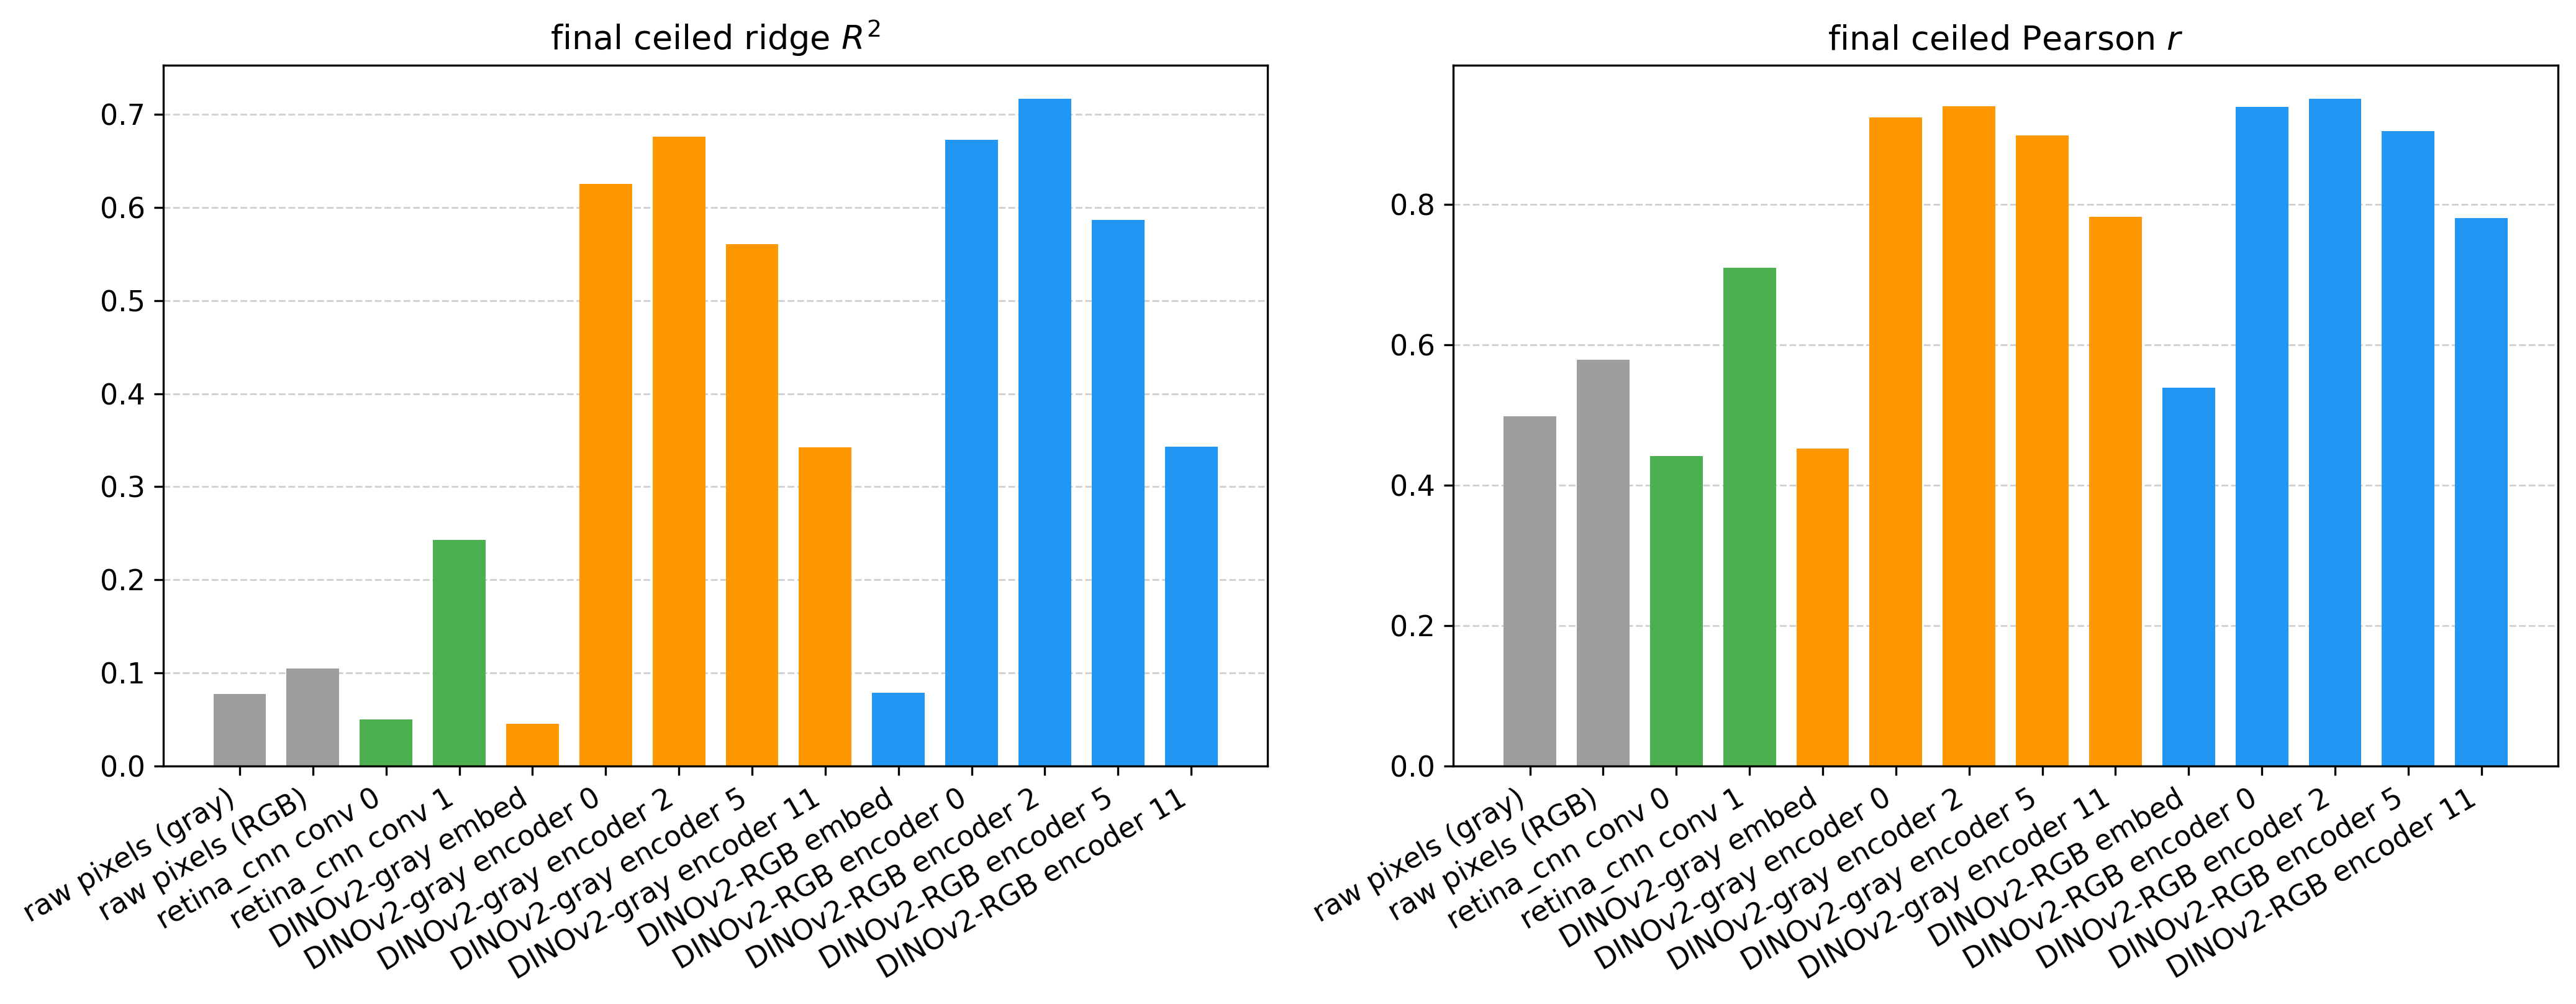
\includegraphics[width=1\textwidth]{figures/overall_match_to_v1.png}
    \caption{Ceiled ridge $R^2$ (left) and ceiled Pearson $r$ (right) for V1 fMRI prediction,
    aggregated across voxels, for raw pixels, prCNN layers, and DINOv2-gray and DINOv2-RGB
    embeddings and encoder layers.}
    \label{fig:overall_v1}
\end{figure}


\noindent Figure~\ref{fig:per_voxel_v1} illustrates this advantage at a
more granular, per-voxel level. It can be observed that
better-matching layers have less spread in their distributions than
worse-matching layers. This tighter spread indicates
that layers with better mean alignment for V1 match V1
more consistently across the entire recording region. Note that
unceiled metrics are used for this per-voxel analysis because a few
voxels have noise ceilings so low that ceiling correction causes
numerical instability, which would artificially widen the spread of
datapoints too much and obscure clarity for analysis.
\begin{figure}[tbp]
    \centering
    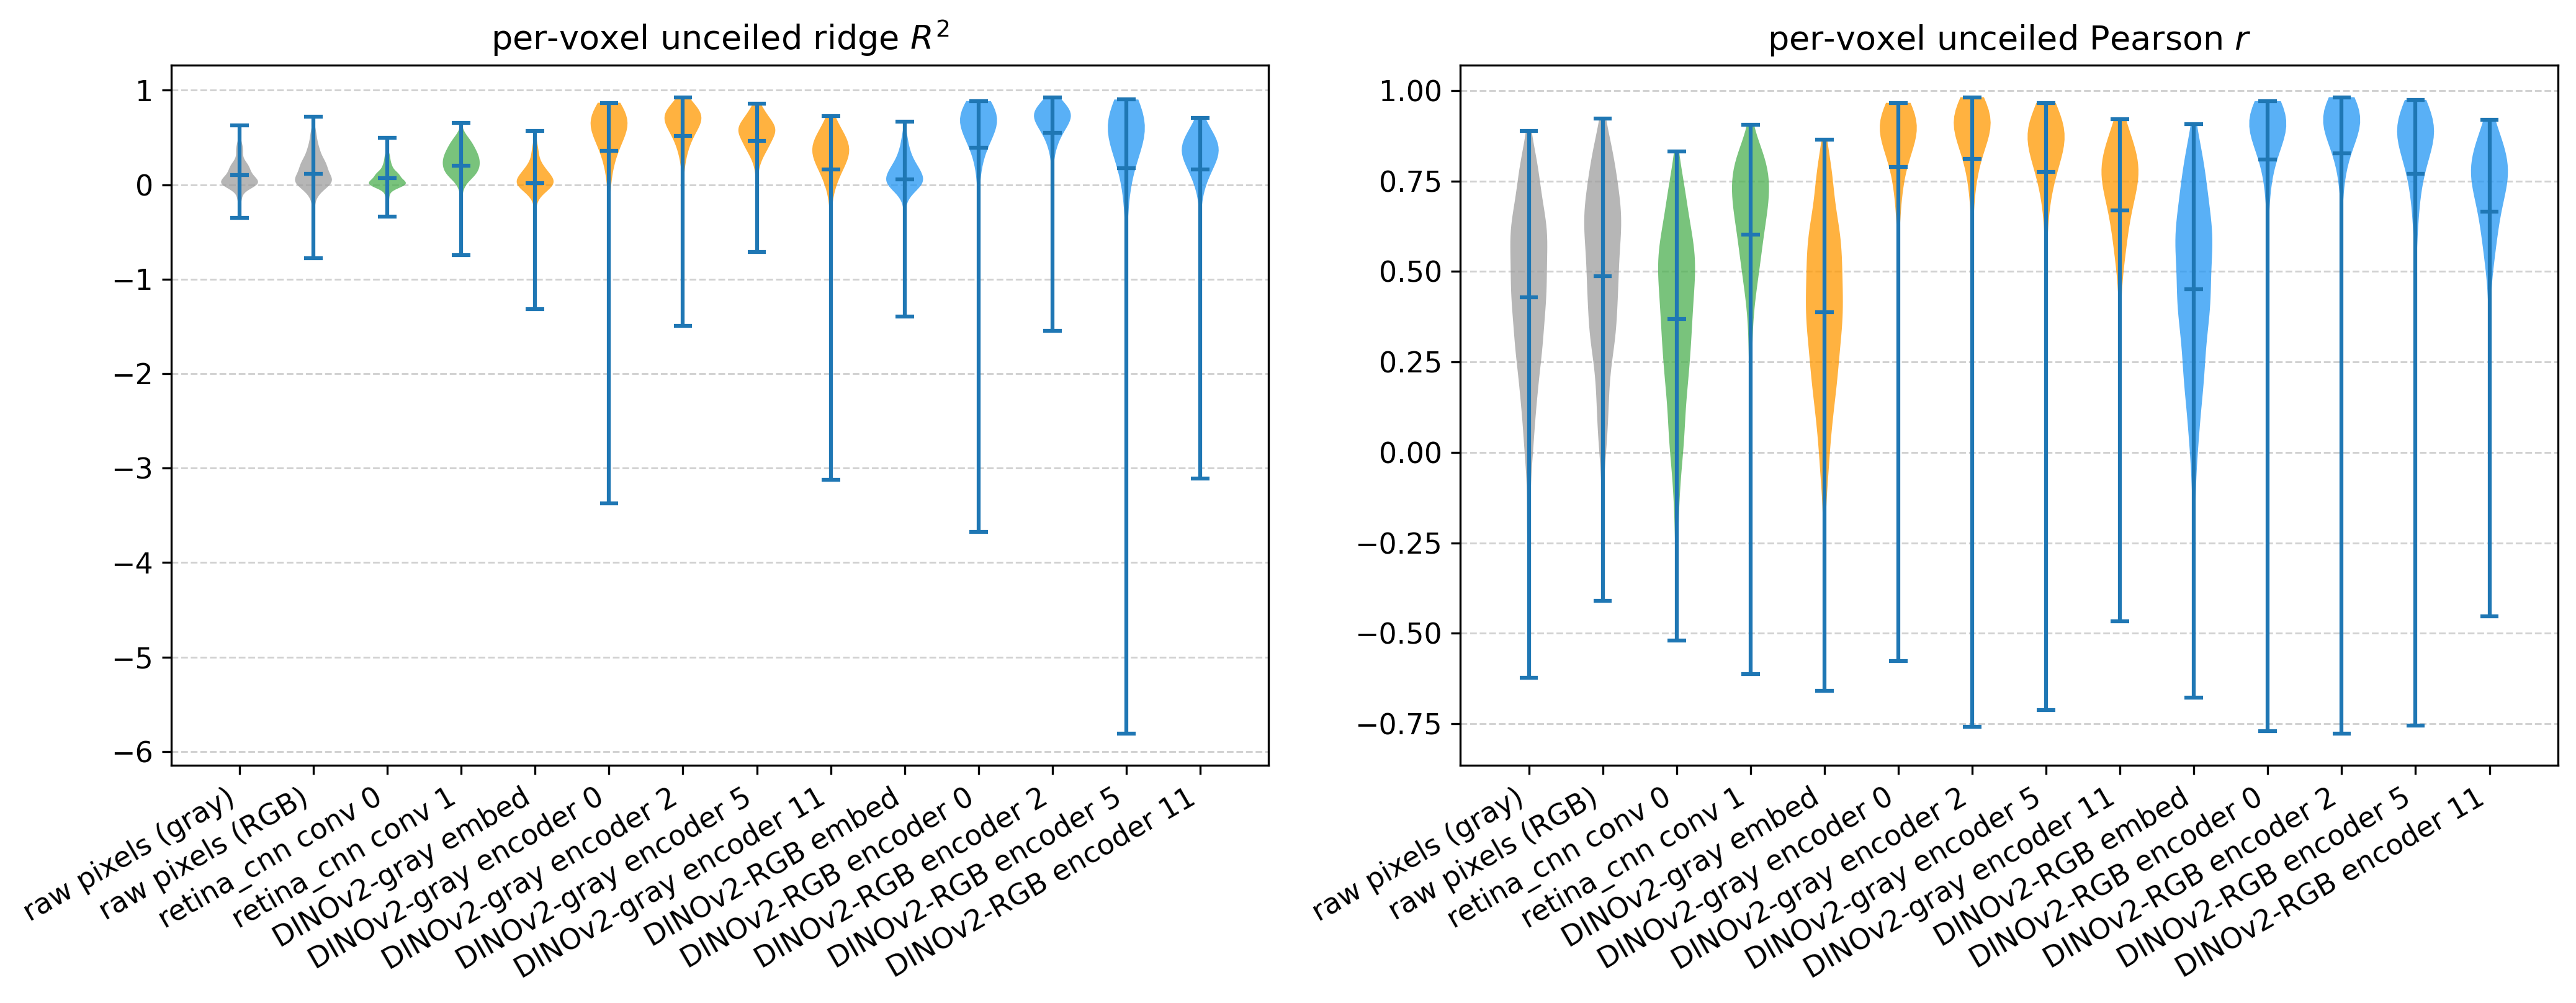
\includegraphics[width=1\textwidth]{figures/per_voxel_match_to_v1.png}
    \caption{Per-voxel distributions of unceiled ridge $R^2$ (left) and unceiled Pearson $r$
    (right) for V1 fMRI prediction, across raw pixels, prCNN (\texttt{conv0}, \texttt{conv1}),
    and DINOv2-gray and DINOv2-RGB embeddings and encoder layers.}
    \label{fig:per_voxel_v1}
\end{figure}

The variance partitioning analysis (Figure~\ref{fig:unique_var})
extends the per-voxel analysis to identify if there are certain
voxels for which the prCNN predicts better than DINOv2 and vice versa. The
results show that DINOv2 outperforms the prCNN across almost all voxels.
DINOv2-RGB encoder~2 versus prCNN \texttt{conv1} yields 91.7\% of voxels
with higher unique variance for DINOv2; DINOv2-gray encoder~2 yields 91.1\%.
Focusing specifically on the voxels for which the unique variance of each
model is positive, literally all of them have higher unique variance for
DINOv2 than the prCNN.
This further strengthens the argument that DINOv2 is better than the prCNN for
aligning with V1 across the entire cortical region. 
\begin{figure}[tbp]
    \centering
    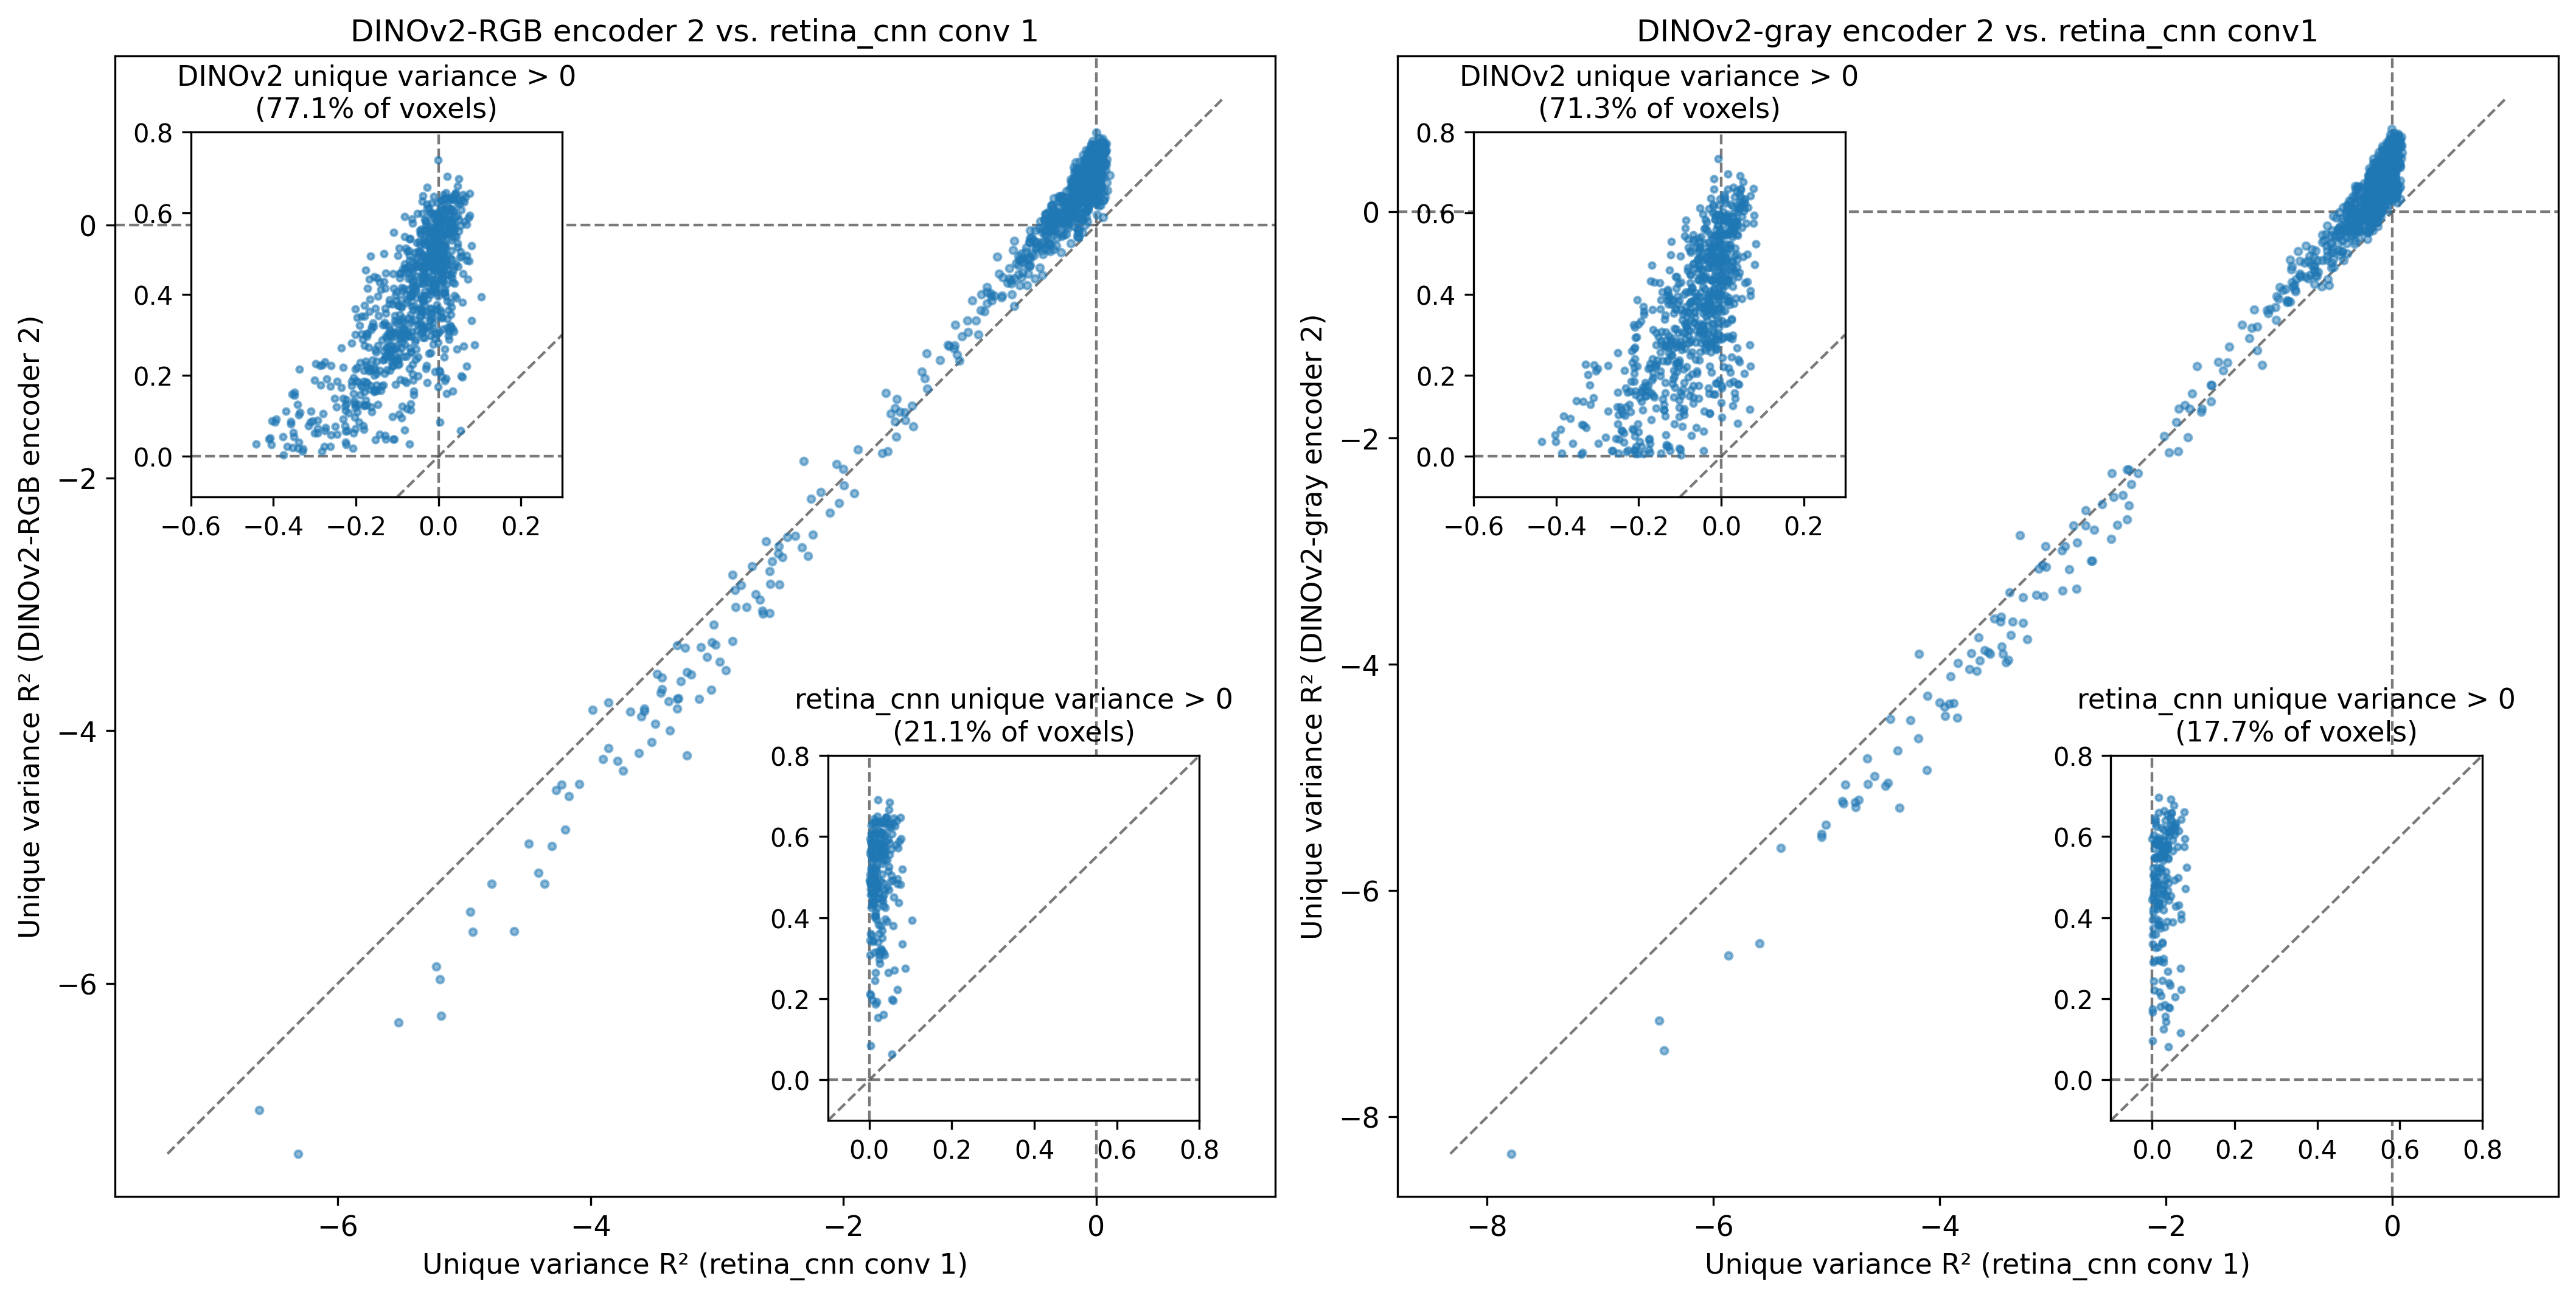
\includegraphics[width=1\textwidth]{figures/per_voxel_unique_var.png}
    \caption{Per-voxel unique variance ($R^2$) from variance partitioning: prCNN
    (\texttt{conv1}) versus DINOv2-RGB encoder~2 (left) and DINOv2-gray encoder~2 (right),
    with identity and zero-reference lines and insets for voxels with positive unique
    variance on each axis.}
    \label{fig:unique_var}
    \end{figure}

\subsection{Step 2: Cross-Model Analysis (Retinal Encoding in DINOv2)}

When directly comparing the models using Linear CKA, ridge
regression, and RSA (Spearman $r$ between cross-model RDMs), this
study finds that the "retina" in DINOv2 corresponds to its very
initial processing stages. Specifically, as shown in
Figure~\ref{fig:match_across_layers}, a broad coarse sweep across all
of DINOv2 reveals that encoder~0 is almost always the best
retina-matching layer, regardless of the metric analyzed (with the
minor exception of \texttt{conv0} versus DINOv2-gray on RSA, where
the preceding embeddings layer performs best with $r = 0.44$). For
\texttt{conv0} versus DINOv2-RGB, encoder~0 attains CKA = 0.31,
RSA $r$ = 0.32, and ridge $R^2$ = 0.29--0.30 (retina$\to$DINOv2 and
DINOv2$\to$retina respectively), compared to CKA $\leq$ 0.21 and
RSA $r \leq$ 0.21 for encoders 2 and deeper.
For the same prCNN layer, DINOv2 given grayscale stimuli shows a
better match than DINOv2 given RGB stimuli (e.g.\ RSA $r$ = 0.44 vs.\
0.32 for \texttt{conv0} at the best encoder-0/embeddings layer), which
is expected since the prCNN is trained exclusively on grayscale images.
Furthermore, for the same DINOv2 layer, \texttt{conv0} matches better
than \texttt{conv1} (e.g.\ CKA = 0.31 vs.\ 0.26 at encoder~0 for RGB).
This is likely because \texttt{conv0} is closer to the raw input
images that DINOv2 is more familiar with, whereas \texttt{conv1} is
more specialized to retinal activity that DINOv2 was never exposed
to. For both retinal layers, similarity drops off sharply in
subsequent transformer blocks---by encoder~7, CKA falls to $\approx 0.09$
and ridge $R^2$ drops to near zero, and by encoders 8--11
all metrics approach zero or become negative---indicating that retinal
features are rapidly transformed into higher-level representations
early in the network of DINOv2.
\begin{figure}[H]
    \centering
    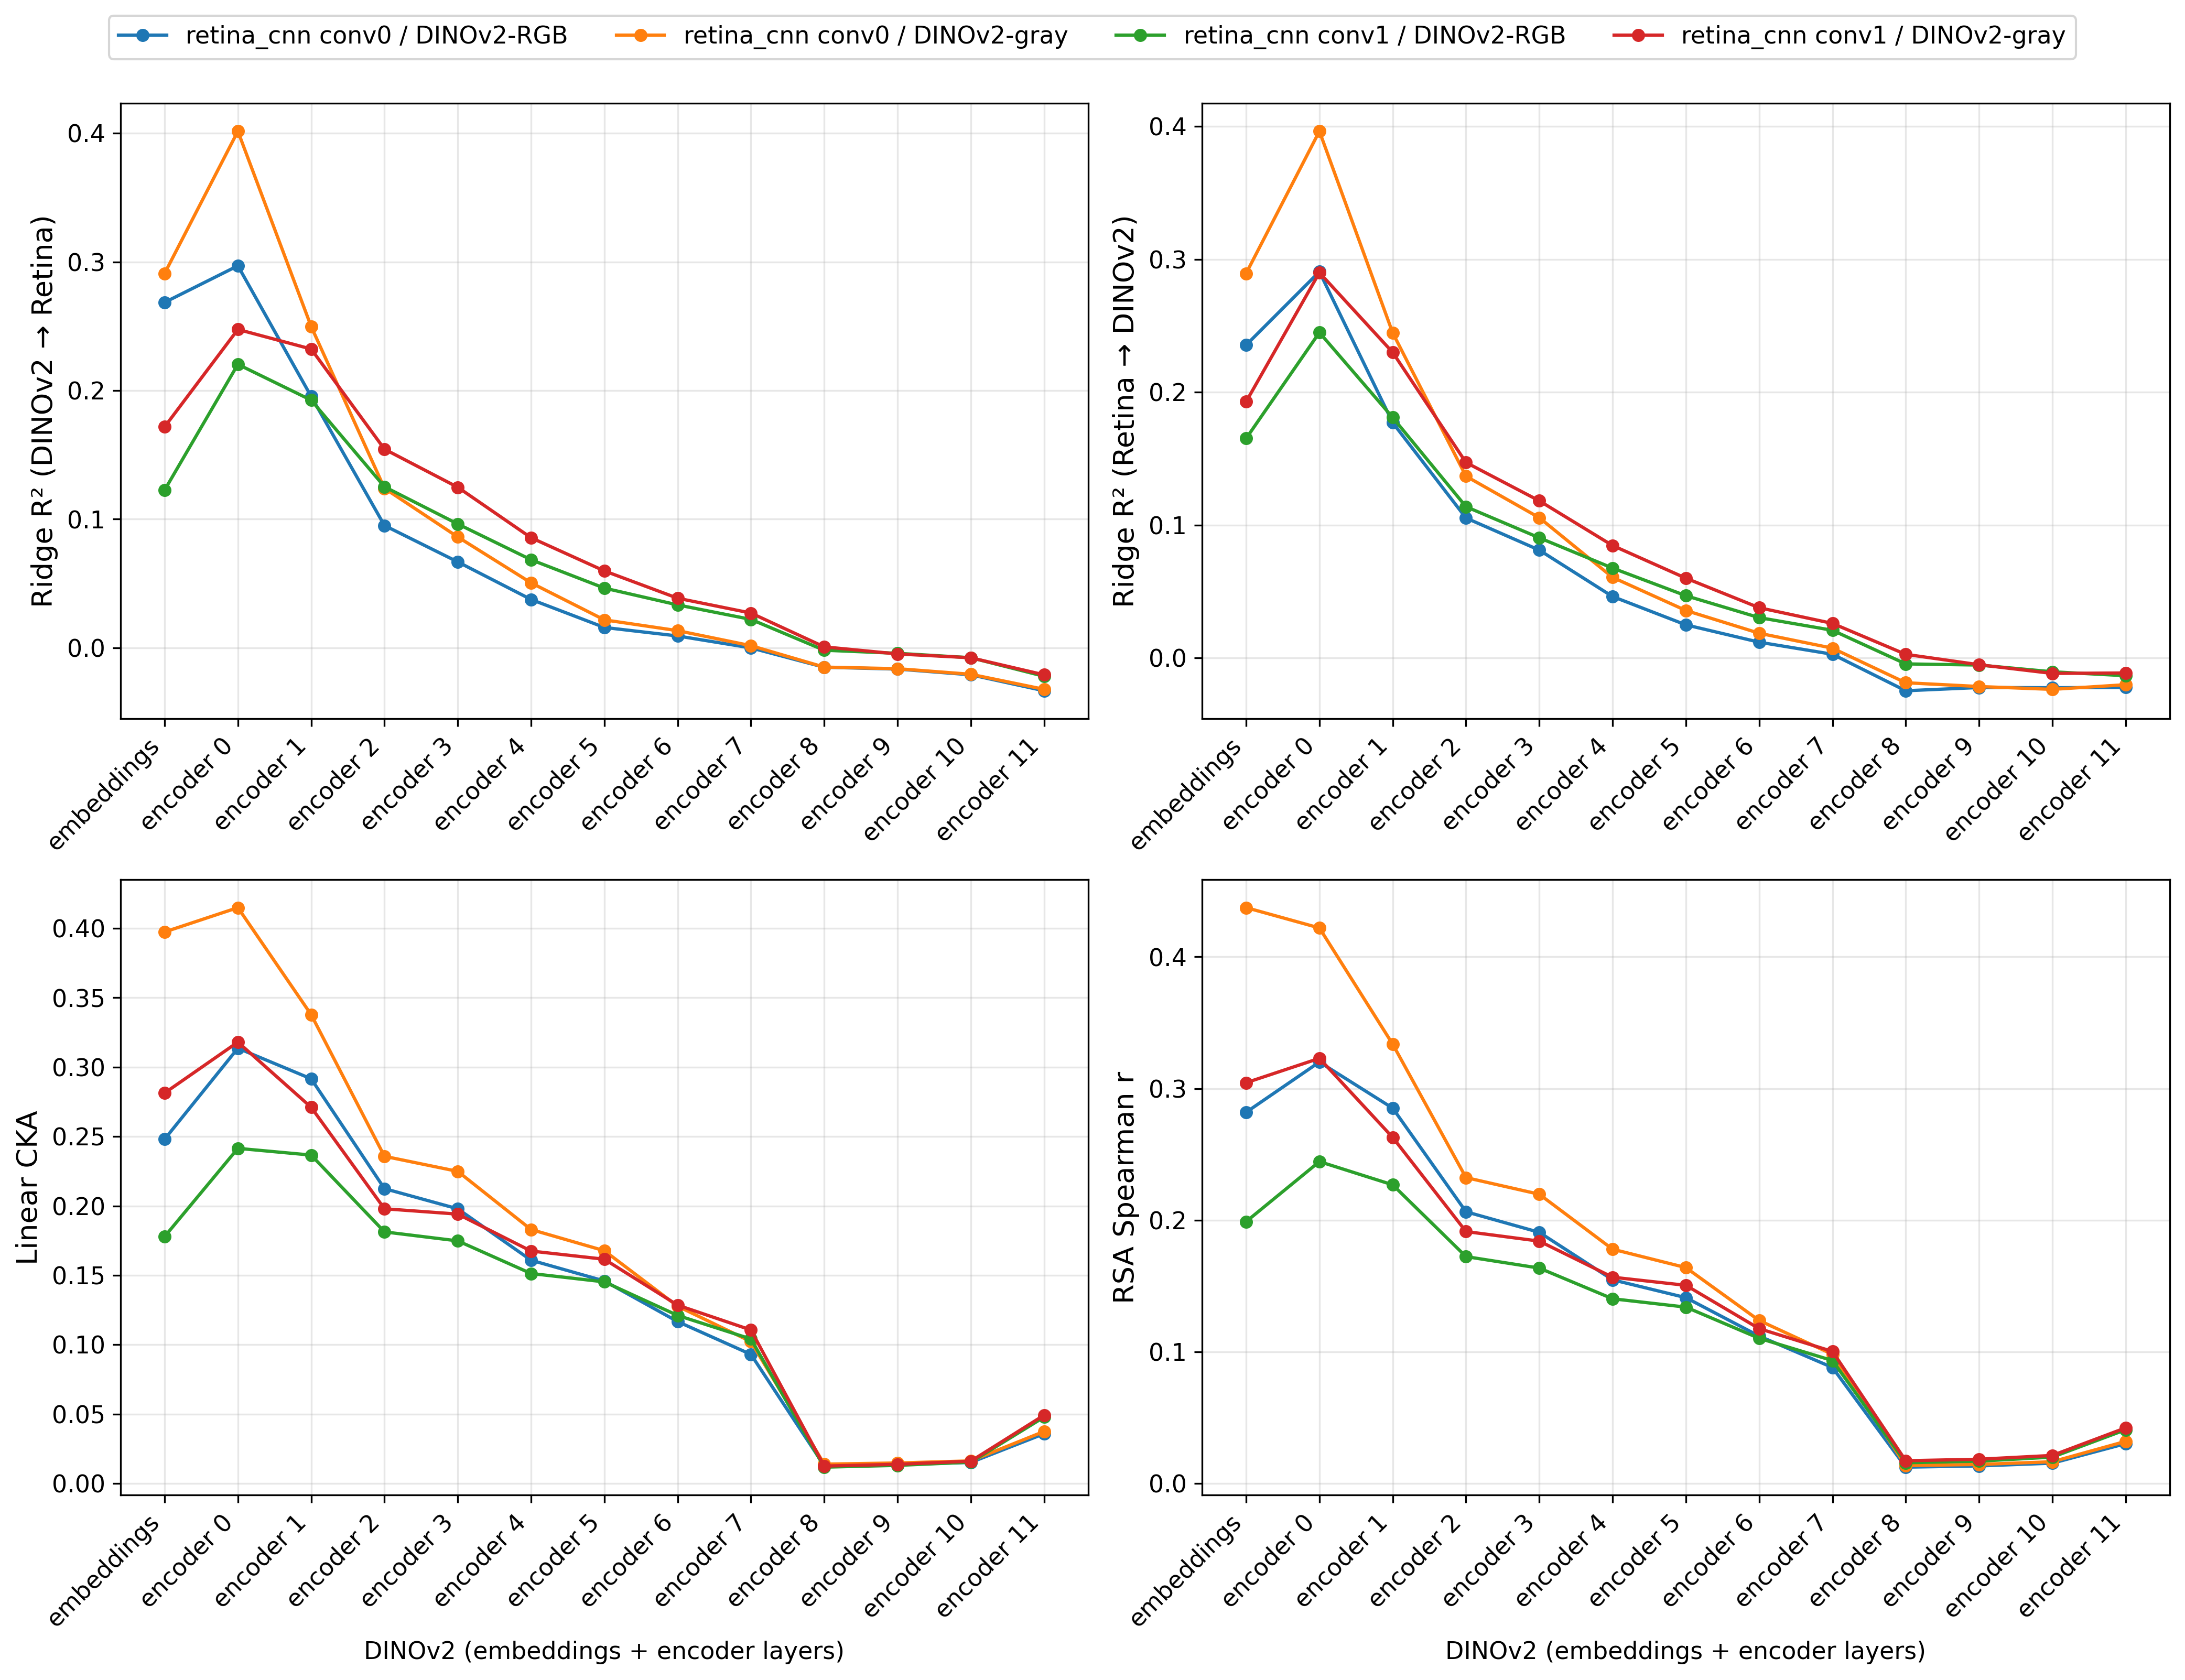
\includegraphics[width=1\textwidth]{figures/match_across_layers.png}
    \caption{Cross-model metrics between prCNN \texttt{conv0}/\texttt{conv1} and DINOv2
    (embeddings through encoder~11): ridge $R^2$ with DINOv2 predicting retina (top left)
    and retina predicting DINOv2 (top right), linear CKA (bottom left), and RSA Spearman $r$
    (bottom right). Curves compare RGB and grayscale DINOv2 for each retinal layer.}
    \label{fig:match_across_layers}
\end{figure}

Having identified encoder 0 as the best match to the retina, this
study takes a closer look at its sublayers (alongside the preceding
embeddings layer) to find exactly where the retina is best
represented. Figure~\ref{fig:cka_sublayers} reports the
corresponding metrics.
\begin{figure}[tbp]
    \centering
    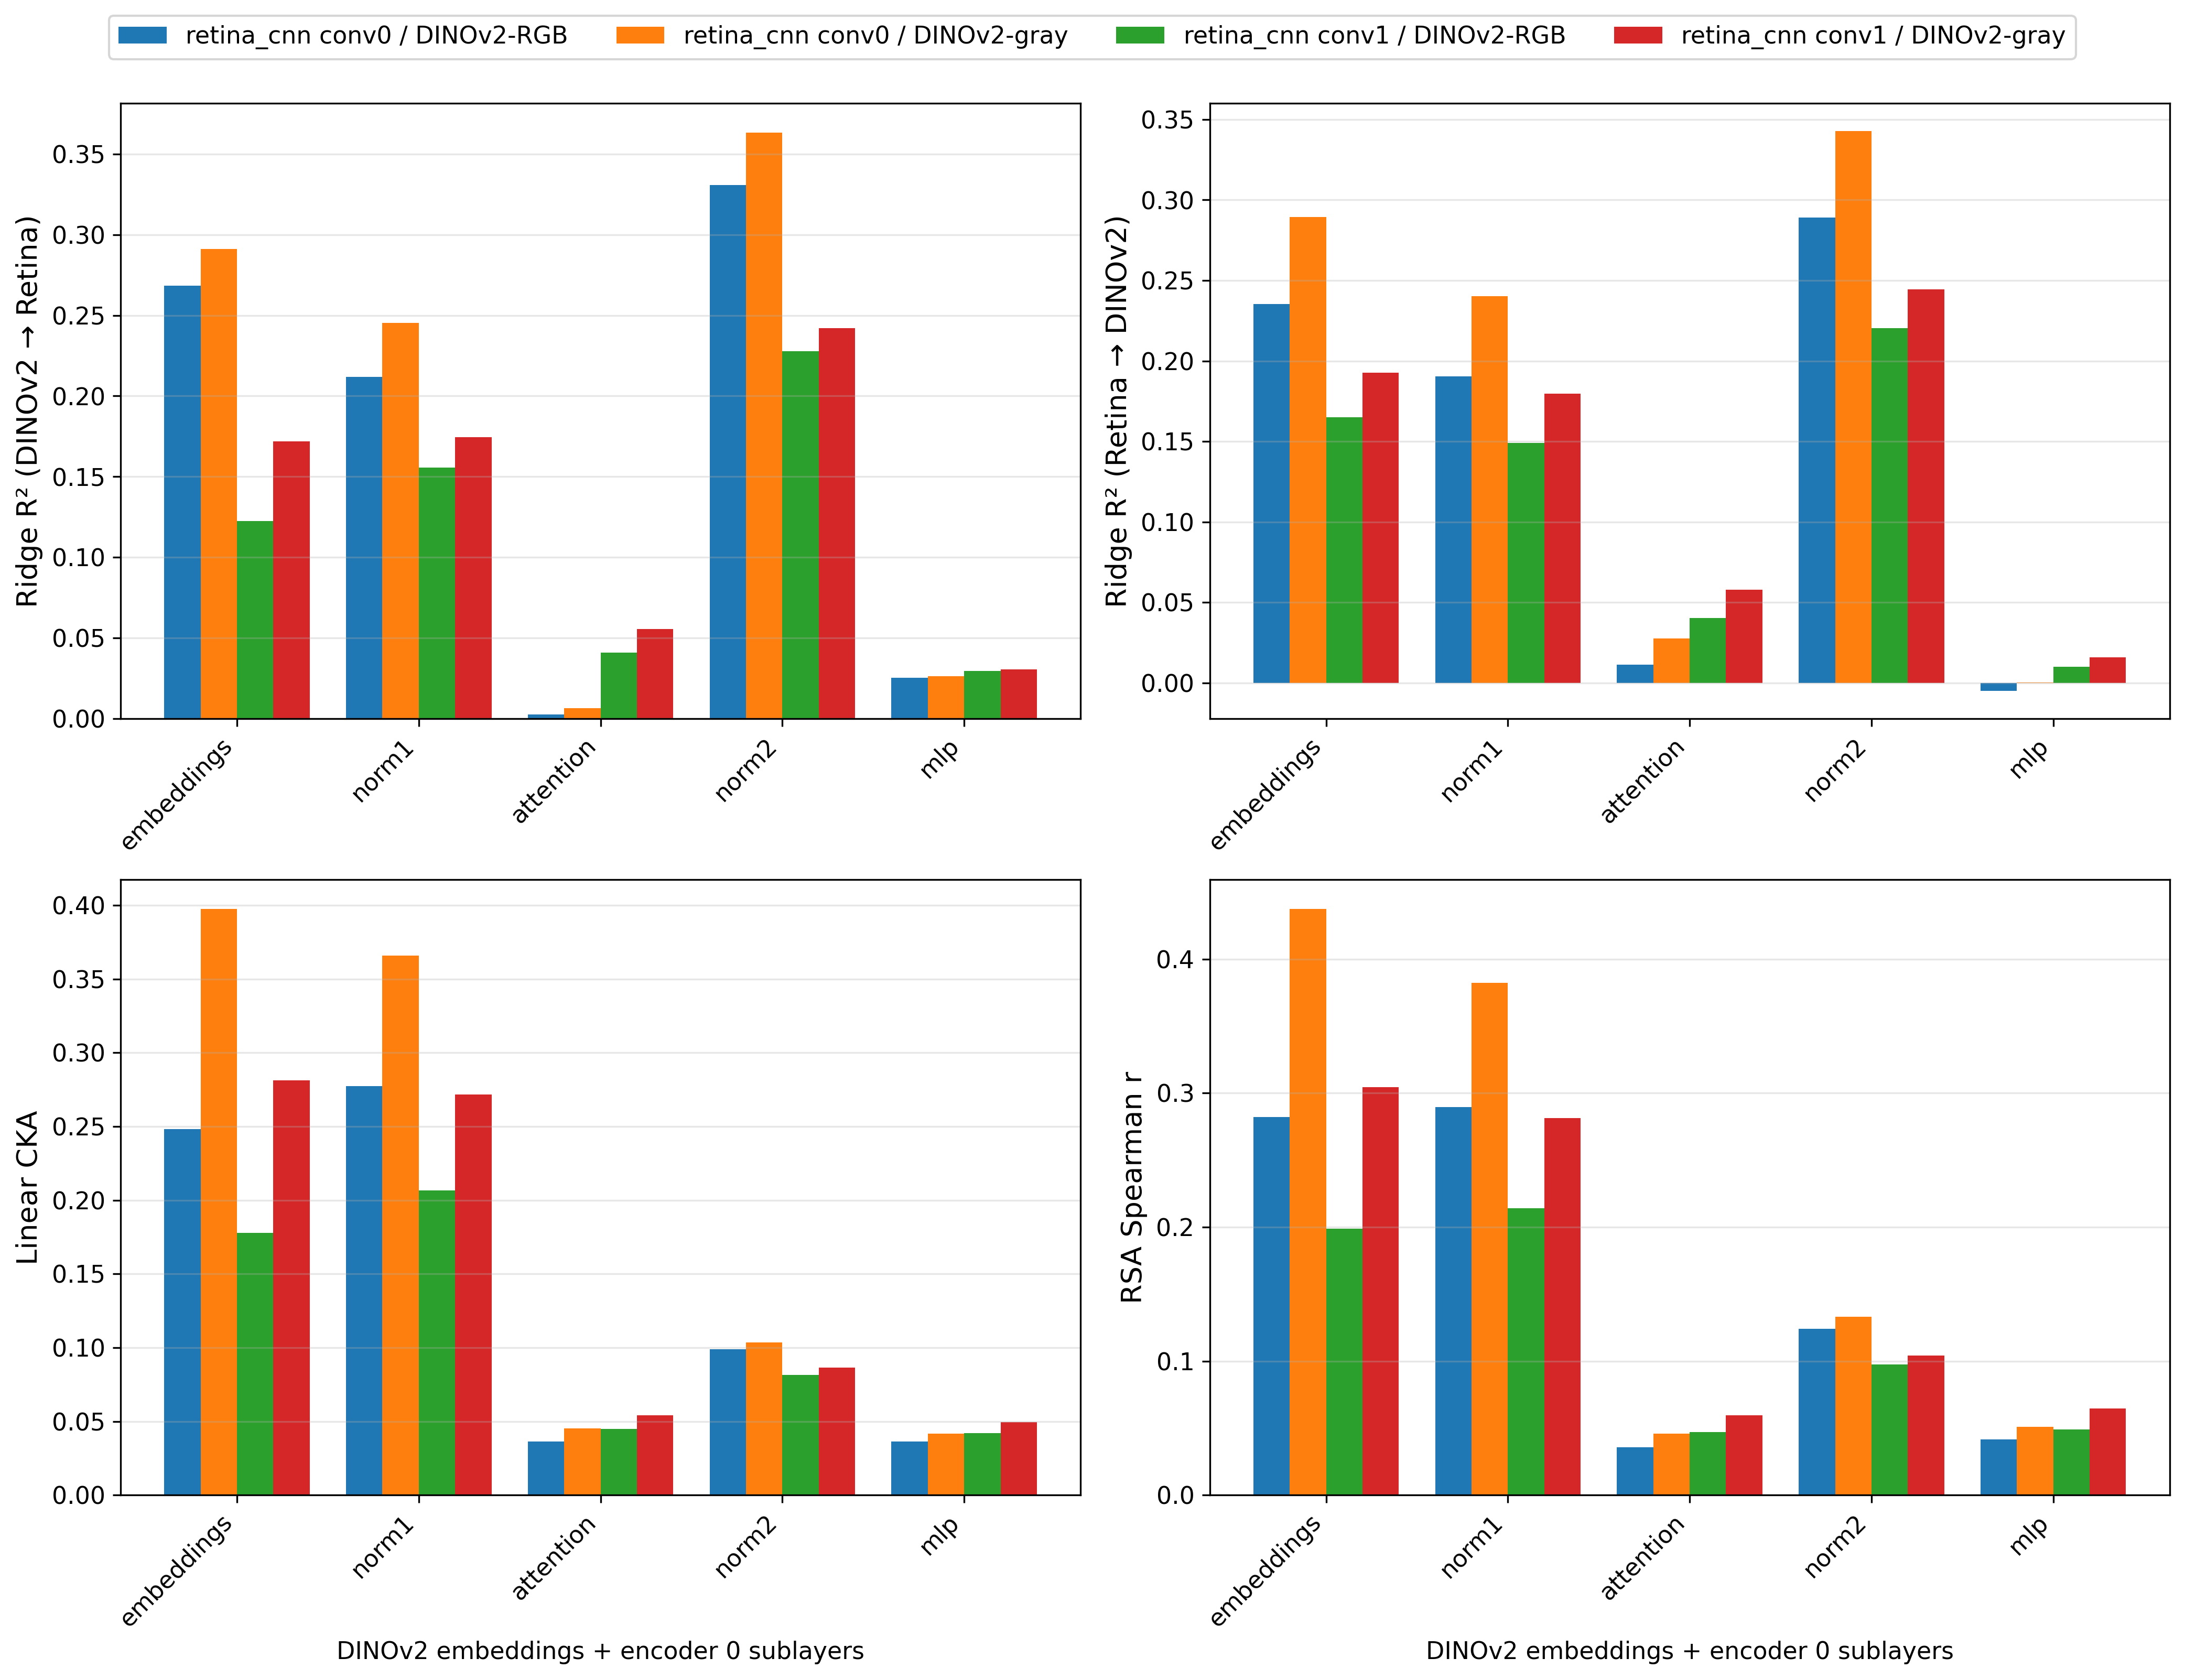
\includegraphics[width=1\textwidth]{figures/match_encoder0_sublayer.png}
    \caption{Bar charts of ridge $R^2$ (DINOv2 $\rightarrow$ Retina, and Retina $\rightarrow$ DINOv2),
    linear CKA, and RSA Spearman $r$ between prCNN \texttt{conv0}/\texttt{conv1} and DINOv2
    embeddings layer and encoder block~0 sublayers (\texttt{norm1}, \texttt{attention}, \texttt{norm2}, \texttt{mlp}),
    for RGB and grayscale DINOv2.}
    \label{fig:cka_sublayers}
\end{figure}

DINOv2-gray matches better across all sublayer conditions. For the
retina layers, \texttt{conv0} matches better for embeddings
and norm sublayers, while \texttt{conv1} matches relatively better
for \texttt{attention} and \texttt{mlp} sublayers.
Embeddings and \texttt{norm1} are nearly identical across all four
metrics, proving that \texttt{norm1} is effectively a pass-through.
\texttt{conv0} matches embeddings slightly better, while
\texttt{conv1} matches \texttt{norm1} slightly better; however, the
gap between embeddings and \texttt{norm1} is small compared to the
drop-off to \texttt{attention} and \texttt{mlp} (and also \texttt{norm2}
in the case of Linear CKA and RSA Spearman $r$).
For example, for \texttt{conv0} vs.\ DINOv2-gray, the
embeddings and \texttt{norm1} share nearly the same CKA ($\approx 0.37$
and RSA $r \approx 0.44$), while \texttt{attention} drops to CKA $\approx 0.26$
and \texttt{mlp} to CKA $\approx 0.24$.
For Ridge $R^2$, \texttt{norm2} is the highest-matching sublayer overall;
for Linear CKA and RSA Spearman $r$, however, \texttt{norm2} drops to
near \texttt{attention} and \texttt{mlp} levels. This divergence
occurs because \texttt{norm2} contains both residual (embedding) and
attention information; Ridge $R^2$ benefits from the richer feature
set, while CKA and RSA penalize the structural distortion introduced by attention.

\section{Analysis}
The results strongly support this study's hypotheses, revealing
distinct insights into both the computational gap between the retina
and V1, and the emergence of retinal-like representations in
self-supervised vision transformers.

\subsection{Step 1: V1 Match Alignment}
The finding that DINOv2 vastly outperforms the prCNN in
predicting V1 activity indicates that subcortical processing—from the
retina, through the LGN, to V1—plays a highly significant role in
transforming visual representations. The prCNN's \texttt{conv0}
maps structurally to photoreceptors and bipolar cells, which perform
minimal processing of raw pixels. Meanwhile, \texttt{conv1} maps to
RGCs, which possess receptive fields and perform preliminary local
visual processing. However, due to the simplicity of the biological
retina (and the corresponding prCNN), visual information
is only processed very locally, falling far short of the
sophistication of V1.

In contrast, DINOv2 encoder 2 best represents V1, and all four
investigated DINOv2 encoder layers outperform all prCNN layers. This is
likely because every transformer encoder layer contains attention
mechanisms that integrate information globally across the entire
visual field. This global integration is a much better match for the
higher-level cortical processing that occurs in the visual pathway
compared to the strictly local processing of the retina and prCNN.

\subsection{Step 2: Cross-Model Alignment}
In the cross-model analysis, the overall alignment values across all
metrics are relatively modest. This is most likely attributed to the
inherent differences in objective functions: the prCNN is
architecturally designed and explicitly trained to match biological
neural activity in the retina, whereas DINOv2 is trained via
self-supervision on image datasets, a task the biological retina does
not perform.

Despite these modest absolute values, the relative patterns are
highly informative. Embeddings and \texttt{norm1} layers are
structurally the most similar to the prCNN. This occurs because
the layer normalization operation is an affine rescaling that largely
preserves upstream representations, acting essentially as a
pass-through for the patch embeddings. The embeddings themselves are
local linear projections of image patches, which is analogous to the
local processing of the retina. Once the network reaches the
attention layers and begins integrating information across the entire
visual field, the representations diverge significantly from retinal
processing.

The pass-through nature of the normalization layers also explains the
sublayer matching patterns. Because \texttt{norm1} preserves the raw
embedding, it is the best match for \texttt{conv0}, which itself is
closer to the raw input. Conversely, the \texttt{attention} and
\texttt{mlp} sublayers involve actual computation and spatial
integration; thus, \texttt{conv1}, which performs slightly more sophisticated
processing than \texttt{conv0}, is the relatively better match for
those sublayers. Furthermore, \texttt{norm2} demonstrates an
intriguing metric divergence: it has the highest Ridge $R^2$ because
it contains both embedding and attention information, giving the
regression more predictive material. However, it yields low CKA and
RSA scores because the attention signal distorts the geometric
structure away from retinal representations. This cleanly illustrates
the difference between encoding-based and similarity-based alignment
metrics.

\section{Conclusion}
In conclusion, this study demonstrates that self-supervised Vision
Transformers like DINOv2 are a remarkably strong match for the
primate cortical visual pathway. The V1 matching analysis highlights
the significant computational transformation that occurs between the
retina and V1: DINOv2's encoder 2 best captures V1 variance, and the
fact that all DINOv2 layers up to encoder 2 vastly outperform all
prCNN layers demonstrates that subcortical processing is
substantial and is effectively captured by DINOv2.

Furthermore, this study locates the "retina" of DINOv2 effectively at
its initial embeddings layer. The near-identity of the embeddings and
\texttt{norm1} sublayers confirms that LayerNorm preserves the
embedding representation. The embedding layer itself is a
patch-level linear projection of the input—a local, relatively
unprocessed transformation analogous to the retina's local receptive
field processing. While this is a straightforward conclusion, it is
mechanistically well-motivated given how locally the retina operates,
highlighting the emergence of biologically plausible early visual
representations in self-supervised transformers.

\textbf{Future Directions:}
There are several avenues for future improvement. First of all, for the prCNN,
instead of simply replicating a static input image 50 times across the time
dimension, this study could jitter the images randomly on each frame according to a 2D
Brownian motion to emulate fixational eye saccades. This better follows the
methodology used by Gogliettino et al. \cite{alex_retina_cnn} to capture
natural temporal dynamics, and would provide a more biologically realistic
input stream that more fully captures the temporal dynamics the model was
designed to exploit. 
% Secondly, while this study's analysis identified strong alignment between the
% prCNN and DINOv2's initial embedding and first transformer block, future
% work could explore the specific contributions of the patch versus position
% embeddings to this alignment, further isolating the earliest stages of feature
% extraction. 
Secondly, recordings from subcortical parts of the visual 
pathway like the LGN or models of the LGN would be a valuable 
addition to the analysis to more comprehensively characterize the subcortical 
elements encoded by DINOv2.

\newpage

\bibliographystyle{plainnat}
\bibliography{references}

\end{document}
